\chapter{SUMMARY, LIMITATIONS AND FUTURE DIRECTIONS}

%Hurricane activity has a profound affect on lives and property along the coast.Property damage in the United States averages in the billions of dollars annually. Hence, the frequency and intensity of hurricanes is the topic of much of the current research. Much less work has been done toward understand the relationships of hurricanes across different regions and how these relationships change with climate factors. This dissertation addresses various relational aspects of hurricane activity through the application of network analysis.

\subsection{SUMMARY}

Paragraph 1

Network analysis has been used in a variety of fields to study relational data, but has yet, until now, to be used for characterizing rice injuries from crop health survey data. The big conceptual hurdle was how to represent the set of rice injuries activities in farmers’ fields as a network. The dissertation considers two different approaches to overcome this hurdle. Due to the fact that the main objective is to capture the relationships of rice injuries, the relationships of rice injuries were captured. The present work is largely expository introducing network analysis and showing how it can be applied to possibly better understanding co-occurrence of rice injuries at farmers’ fields. Results of network analysis may offer new insight into pest management with another tool to identify important injuries to be monitored or controlled.

This research was divided into two cases based on the approaches for constructing the network. The first case consisted of networks developed based on the co-occurrence relationships of rice injuries under each production seasons and production environments, and the second case consisted of networks developed based on the differential co-occurrence relationships of rice injuries in different production season and yield levels. 

But before constructing a network, selecting the suitable correlation methods is important because the method that can identify injuries with true concordance support us to gain knowledge from co-occurrence analysis of survey data. The exploratory analysis of crop health survey data reveals that their values of injuries are not normally distributed, with different measurements. In this study, Spearman’s correlation method is the most suitable correlation method because of it robustness to noise and outliers, and ability to accurately capture the interactions. Networks in this study are constructed in three steps. In step 1, selecting data for constructing are obtained. Next, co-occurrence matrix (adjacency matrix) is computed from the selected data using Spearman’s correlation methods, then network graph is drawn by connecting injuries (nodes) that have a non-zero entry in the co-occurrence matrix.

The networks, in the first case present links rice injuries (nodes) and co-occurrence relationships (edges) with Fruchterman-Reingold layout, which placed nodes with stronger and/or more connections closer to each other. Next, the topology (structure) of the network was examined including degree, betweenness, and local clustering coefficient. Paths through the network are routes between nodes via the links. Node degree is defined as the number of links a node has. Betweenness quantify how many shortest paths go through each node. The local clustering coefficient is a measure of the degree to which nodes tend to cluster together. It is defined as how often a node forms a triangle with its direct neighbors, proportional to the number of potential triangles the relevant node can form with its direct neighbors. These measures can be as unified criteria for identifying the importance injuries to be monitored and controlled. For example, nodes with high node degree and betweenness are highly potential involved in the rice fields because they have many connections, and highly co-occur with many injuries, and they can be activated very easily, since a lot of co-occurrence activities flows through them (high betweenness). In this case, networks reveal syndromes (“communities” in term of network) is the group of injuries that relatively closely co-occur with each other. Networks shown in Figure to represent the injury syndromes in the same color.

The second case, differential networks are used for identifying a set of injuries whose significantly changes across two conditions. Therefore, theses network show injuries which are significantly co-occur in specific condition, but not in others. Differential co-occurrence networks of rice injuries in season (dry versus wet season) and in yield level (lower versus higher yield level) are constructed. The topological structures of these networks were again probed using various centrality measures in order to identify the most significant injuries in each network.


\begin{landscape}
\begin{figure}
\centering
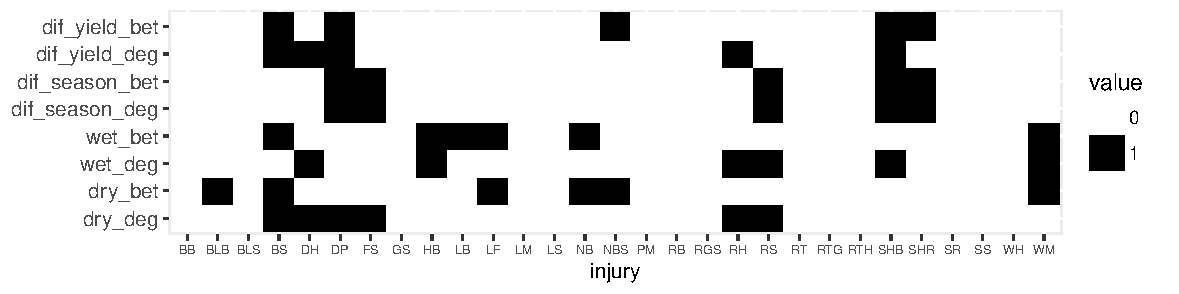
\includegraphics[height = 0.4\textwidth]{figures/sum_mat_CP.pdf}
\caption{Central Plain}
%\label{fig:}
\end{figure}    
\begin{figure}
\centering
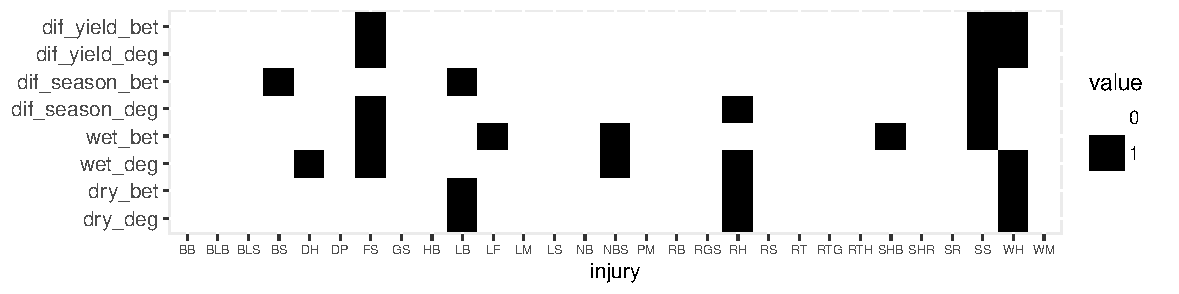
\includegraphics[height = 0.4\textwidth]{figures/sum_mat_OD.pdf}
\caption{Odisha}
%\label{fig:}
\end{figure}    
\end{landscape} 

\begin{landscape}
\begin{figure}
\centering
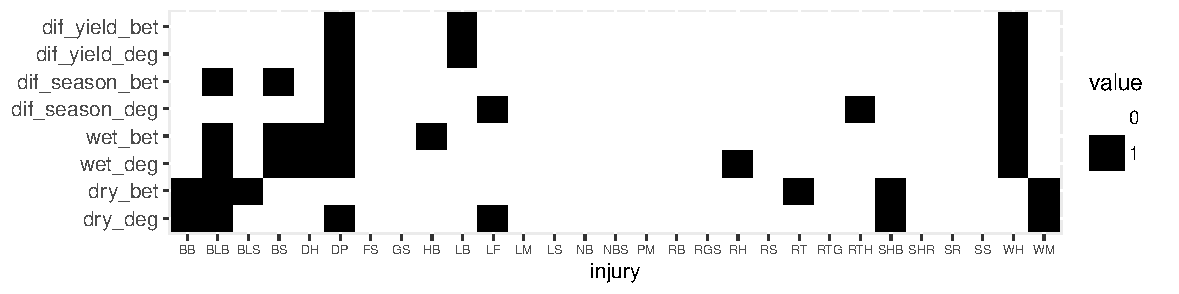
\includegraphics[height = 0.4\textwidth]{figures/sum_mat_RR.pdf}
\caption{Red River Delta}
%\label{fig:}
\end{figure}    
\begin{figure}
\centering
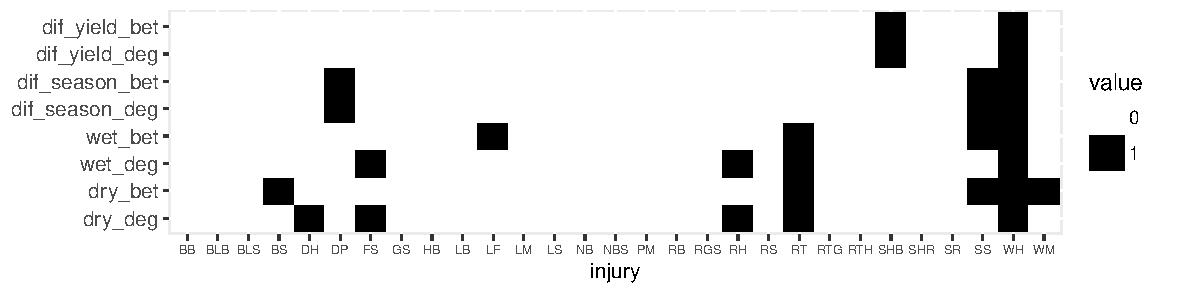
\includegraphics[height = 0.4\textwidth]{figures/sum_mat_TM.pdf}
\caption{Tamil Nadu}
%\label{fig:}
\end{figure}    
\end{landscape} 

\begin{landscape}    
\begin{figure}
\centering
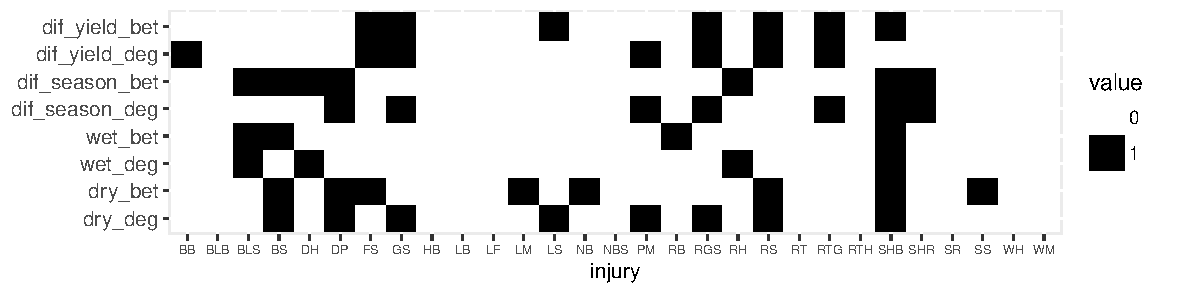
\includegraphics[height = 0.4\textwidth]{figures/sum_mat_WJ.pdf}
\caption{West Java}
%\label{fig:}
\end{figure}    
\end{landscape} 

\newpage
\subsection{LIMITATIONS AND FUTURE DIRECTION}

This dissertation answered the question of how to create a network from a list of hurricane occurrences. However the two approaches taken resulted in undirected networks. That is, the links between nodes do not have a direction of relationship meaning the relationship is symmetric. Consider a hurricane that hits Florida before moving west and hitting Texas. In the above network analysis Texas and Florida are linked in an undirected way. However, since Florida gets hit first it might make sense to create a directed network where the link between Texas and Florida points in the direction of Texas. Similar analysis as was done on the undirected network could then be performed on the directed network with additional characteristics arising about the in and out-node linkages. However, the relatively small number of directed linkages may preclude an in-depth analysis using directed networks.
One way around the relatively small sample size of 158 years is to include older historical data in the analysis. Recent work by Chenoweth (2006) to collate historical archives of tropical cyclones in the western North Atlantic basin back to 1700 is particularly relevant in this regard. Perhaps better still is to include data from paleotempestology studies (Liu and Fearn 1993; Donnelly and Woodruff 2007). Paleotempestology is the study of prehistoric storms from geological and biological evidence. Coastal wetlands and lakes are subject to overwash events during hurricanes, when barrier sand dunes are overtopped by storm surge. A sediment core taken from the bottom of a near-coastal lake or marsh will record these episodic events as sand layers between the organic peat. As Liu (2007) points out, each record serves as a type of climate station. Connecting these various stations together using network analysis could help better understand the relationship between hurricanes and climate (Elsner 2007).
As mentioned in Chapter 4 two regions affected at least once over the period of record by the same hurricane results in a linkage. Information about how frequently this occurs is lost from the type of network analysis. Future research could consider links with various “strengths” depending on how often regions are both affected. The extra information provided by linkage strength would likely add to a better understanding of the hurricane network.
Another direction would be to build prediction models of network structure based on pre–season climate conditions. One way this could be achieved is using a Bayesian network (or a belief network). A Bayesian network (or a belief network) is a probabilistic graphical model that represents a set of variables and their probabilistic independencies. Because a Bayesian network is a complete model for the variables and their relationships, it can be used to answer probabilistic queries about them. For example, the network can be used to find out updated knowledge of the state of a subset of variables when other variables (the evidence variables) are observed. This process of computing the posterior distribution of variables given evidence is called probabilistic inference. The posterior gives a universal sufficient statistic for detection applications, when one wants to choose values for the variable subset which minimize some expected loss function, for instance the probability of decision error. For example, a Bayesian network could represent the probabilistic relationships between diseases and symptoms. Given symptoms, the network can be used to compute the probabilities of the presence of various diseases. In terms of the hurricane network given the landfall location, the network could be used to compute the probabilities of the same hurricane occurring in another location. For the visibility network given the visibility of one year, the network could be used to compute the probabilities of visibility in a future year.
Finally is would be possible to construct visibility networks from the covariate data including the NAO, SST, and ENSO. The structure of these networks could then be compared with the structural properties of the hurricane network. Then each of those network structures could then be examined using local and global metrics. This investigation may provide further insight into how the indices are intra related in addition to being compared and/or conditioned against/on one another.